%----------------------------------------------------------------------------
\section{Bevezetés a Cisco eszközök programozásába 1}
{\footnotesize A forgalomszűrés, forgalomszabályozás (Trafficfiltering, ACL) céljai és beállítása (konfigurációja) egy választott példa alapján.}
%----------------------------------------------------------------------------
\subsection{A forgalomszűrés, forgalomszabályozás (Trafficfiltering, ACL) céljai és beállítása (konfigurációja) egy választott példa alapján.}
A rendszergazdáknak meg kell találniuk annak a módját, hogy megakadályozzák a hálózat
jogosulatlan elérését, miközben a belső felhasználók számára lehetővé teszik a szükséges
szolgáltatások használatát. Bár a biztonsági eszközök, mint például a jelszavak, a visszahívó
berendezések és a fizikai biztonsági eszközök sok segítséget nyújtanak, gyakran nem
rendelkeznek az alapvető forgalomszűréshez szükséges rugalmassággal és a rendszergazdák
igényeinek megfelelő vezérlési lehetőségekkel. Előfordulhat például a hálózati rendszergazda
lehetővé kívánja tenni a felhasználók számára az internet elérését, de nem akarja, hogy külső
felhasználók telnettel hozzáférhessenek a LAN-hoz.

A forgalomirányítók alapvető forgalomszűrési lehetőségeket biztosítanak, például hozzáférési
listákat (access control list, ACL) az internetes forgalom letiltásához. Az ACL engedélyező és
tiltó utasítások sorozata, melyek címekre vagy felsőbb rétegbeli protokollokra alkalmazhatók.
Ebben a modulban a normál és kiterjesztett ACL-ek használatáról, mint a hálózati forgalom
vezérlési módszeréről fogunk tanulni, továbbá arról, hogyan használhatók az ACL-ek
valamilyen biztonsági megoldás részeként.

Ezenkívül a fejezetben tippek, elgondolások, javaslatok és általános útmutatások is
szerepelnek az ACL-ek használatával, valamint a létrehozásukhoz szükséges parancsokkal és
beállításokkal kapcsolatban. Végül a fejezet példákat mutat a normál és a kiterjesztett ACL-
ekre és a forgalomirányítók interfészein történő alkalmazásukra.

Az ACL-ek akár egyetlen sorból is állhatnak, ha a cél egy adott állomásról származó
csomagok továbbításának engedélyezése, de tartalmazhatják szabályok és feltételek rendkívül
összetett halmazát is, amelyek pontosan megadják az engedélyezett forgalom jellegét, illetve
befolyásolják a forgalomirányító folyamatok teljesítményét.

\subsubsection{A hozzáférési listák működésének alapelvei}
Az ACL-ek feltétellisták, amelyek a forgalomirányító interfészén keresztülhaladó forgalomra
vonatkozóan lépnek érvénybe. Ezek a listák írják elő a forgalomirányító számára, hogy a
csomagokat fogadja el vagy utasítsa vissza. Az elfogadás és a visszautasítás meghatározott
feltételek alapján is történhet. Az ACL-ek segítségével lehetővé válik a forgalom felügyelete,
valamint a hálózatról kiinduló és az oda befutó elérések biztonságossá tétele.

ACL-ek minden irányított protokollhoz létrehozhatók, többek közt az internetprotokollhoz
(IP) és a hálózatközi csomagcseréhez (IPX) is. Az ACL-ek a forgalomirányítón konfigurálva
adott hálózat vagy alhálózat elérhetőségének vezérlésére használhatók.

Az ACL-ek úgy szűrik a hálózati forgalmat, hogy az irányított csomagok továbbítását vagy
eldobását írják elő a forgalomirányító interfészein. A forgalomirányító minden csomagot
megvizsgál annak meghatározásához, hogy azt az ACL-ben meghatározott feltételek szerint
továbbítani vagy eldobni kell. Az ACL-ek a forrás- és a célcímekre, a protokollokra és a
felsőbb rétegbeli portszámokra nézve adnak meg feltételeket.

Az ACL-eket protokollonként, irányonként és portonként kell létrehozni. Ha szabályozni
szeretnénk egy adott interfész forgalmát, akkor a rajta engedélyezett protokollok
mindegyikéhez külön ACL-t kell készíteni. Egy ACL egy interfészen egyszerre csak egy
irány forgalmát szabályozza. Minden irányhoz külön ACL-t kell létrehozni, egyet a kimenő,
egyet pedig a bejövő forgalomhoz. Végül minden interfészen több protokoll és irány is
definiálható. Ha például egy forgalomirányítónak két interfésze van, és ezeken IP, AppleTalk
és IPX alapú forgalom zajlik, akkor 12 külön ACL-t kell rajta létrehozni: minden
protokollhoz egy-egy ACL, szorozva kettővel a kimenő és a bejövő forgalom miatt, szorozva
kettővel, vagyis a portok számával.

ACL-eket többek között a következő okok miatt szokás létrehozni:
\begin{enumerate}[nosep]
	\item Korlátozható a hálózat forgalma, és növelhető a teljesítménye.
	\item Biztosítják a forgalom szabályozását.
	\item Az útvonalfrissítések továbbítása is korlátozható. Ha a hálózati környezet miatt nincs szükség a frissítésekre, sávszélességet lehet megtakarítani.
	\item Alapszintű hálózati hozzáférés-szabályozást biztosítanak. Az ACL-ek engedélyezhetik például a hálózat egy részének elérését egy állomás számára, és megtilthatják egy másiknak. Lehetséges például, hogy az A állomás hozzáférhet a személyzeti osztály hálózatához, míg a B állomásnak ezt megtiltjuk.
	\item Eldönthetjük, hogy milyen típusú forgalom továbbítódjon és milyen törlődjön a forgalomirányító interfészein. Például engedélyezhetjük az elektronikus levelek továbbítását, de a telnetet tilthatjuk.
	\item A rendszergazdák szabályozhatják, hogy az ügyfelek a hálózat mely részeihez férhetnek hozzá.
	\item Ki lehet választani bizonyos állomásokat, és számukra engedélyezni vagy megtiltani a hálózat egy részének elérését.
	\item A felhasználók számára engedélyezni vagy tiltani lehet bizonyos szolgáltatások, például az FTP vagy a HTTP elérését.
\end{enumerate}

Ha egy forgalomirányítón nincsenek ACL-ek megadva, akkor a forgalomirányítóba befutó csomagok mindegyike továbbhaladhat a hálózat bármely része felé.
\begin{figure}[h]
	\centering
	\begin{subfigure}{0.45\linewidth}
		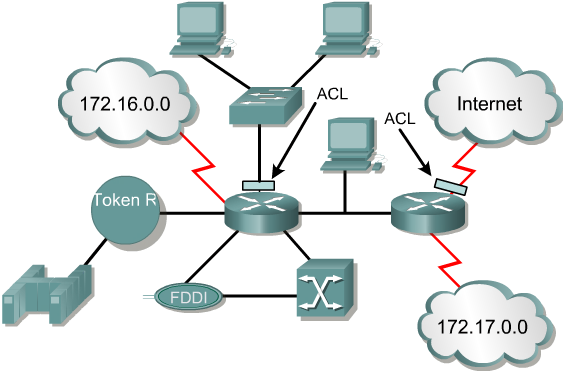
\includegraphics[width=\linewidth]{fig/16-ACL}
		\caption{}
	\end{subfigure}
	\begin{subfigure}{0.45\linewidth}
		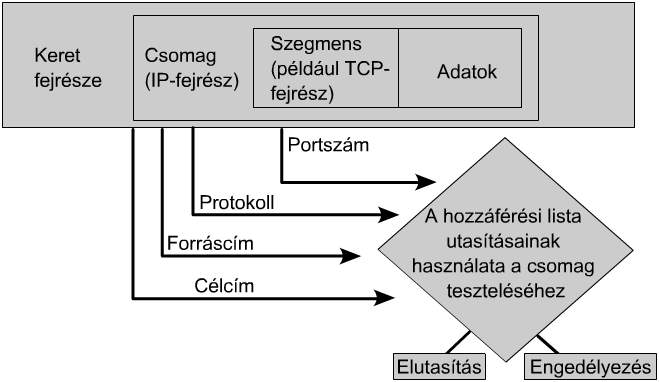
\includegraphics[width=\linewidth]{fig/16-ACL_list-schema}
		\caption{}
	\end{subfigure}
	\caption{}
\end{figure}

\subsubsection{ACL-ek létrehozása}
Az ACL-ek létrehozása globális konfigurációs módban történik.
Számos különböző típusú ACL létezik, így normál, kiterjesztett, IPX, AppleTalk stb. ACL.
Amikor egy forgalomirányítón ACL-eket konfigurálunk, akkor egy-egy szám
hozzárendelésével mindegyiket egyértelműen azonosítanunk kell. A szám megadja az ACL
típusát; ebből következően az adott típushoz tartozó értéktartományba kell esnie:\\
\begin{tabular}{l|l}
	\hline 
	\rule[-1ex]{0pt}{2.5ex} Protokoll & Tartomány \\ 
	\hline 
	\rule[-1ex]{0pt}{2.5ex} IP & 1-99, 1300-1999, 2000-2699 \\ 
	\hline 
	\rule[-1ex]{0pt}{2.5ex} Kiterj. IP & 100-199, 2000-2699 \\ 
	\hline 
	\rule[-1ex]{0pt}{2.5ex} AppleTalk & 600-699 \\ 
	\hline 
	\rule[-1ex]{0pt}{2.5ex} IPX & 800-899 \\ 
	\hline 
	\rule[-1ex]{0pt}{2.5ex} Kiterj. IPX & 900-999 \\ 
	\hline 
	\rule[-1ex]{0pt}{2.5ex} IPX szolgáltatáshirdetés (SAP) & 1000-1099 \\ 
	\hline 
\end{tabular}\\

Miután beléptünk a megfelelő parancsmódba és eldöntöttük, hogy milyen típusú listát
szeretnénk létrehozni, az \verb|access-list| paranccsal, illetve a szükséges paraméterek segítségével
kell megadnunk a hozzáférési lista utasításait.\\
A hozzáférési listák létrehozása az első lépés.\\
A második végrehajtandó művelet a listák hozzárendelése a megfelelő interfészekhez.\\

Az ACL definiálása a következő paranccsal:\\
\verb|Router(config) #access-list access-list-number {permit / deny test-conditions}|

\paragraph{1. lépés:} Az ACL-t egy globális utasítás azonosítja. A normál IP-címekhez az 1-99 tartomány van
fenntartva. Ez a szám mutatja az ACL típusát. A Cisco lOS 11 .2-es verziójától kezdődően az
ACL-ekhez nem csak szám, de név is rendelhető, például oktatasi\_csoport. A globális ACL
utasítás permit illetve deny kifejezése adja meg, hogy a Cisco lOS szoftver hogyan kezelje a
tesztfeltételeket kielégítő csomagokat. A permit általában azt jelenti, hogy a csomag
használhat egy vagy több - később meghatározandó - interfészt. A záró kifejezés(ek) az ACL
állítás által használandó tesztfeltételeket adják meg.

\paragraph{2. lépés:} Ezután alkalmazni kell az ACL-eket egy interfészre az \verb|access-group| paranccsal.\\
Példa: \verb|Router (config-if) #{protocol) access-group access-list number|\\
A hozzáférési lista számával azonosított összes ACL utasítás hozzárendelődik egy vagy több
interfészhez. Az ACL tesztfeltételeket kielégítő csomagok a hozzáférési csoport bármely
interfészét használhatják.

TCP/IP használata esetén az ACL-eket egy vagy több interfészhez lehet hozzárendelni.
Az \verb|ip access-group| parancs segítségével a bejövő vagy a kimenő forgalom szűrésére
állíthatjuk be.

\begin{verbatim}
	Router(config)#access-list 2 deny 172.16.1.1
	Router(config)#access-list 2 permit 172.16.1.0 0.0.0.255
	Router(config)#access-list 2 deny 172.16.0.0 0.0.255.255
	Router(config)#access-list 2 permit 172.0.0.0 0.255.255.255
	Router(config) #interface ethernet 0
	Router(config)#ip access-group 2 in
\end{verbatim}

Az access-group parancsot interfészkonfigurációs módban kell kiadni.
Amikor egy ACL-t hozzárendelünk egy interfészhez, akkor ki kell választanunk, hogy a
bejövő vagy a kimenő forgalomra vonatkozzon. A szűrés tehát az adott interfészre beérkező
és a róla távozó csomagokra vonatkozhat. Annak megállapításához, hogy az ACL a bejövő
vagy a kimenő forgalmat szűrje, az egyes interfészeket a forgalomirányító belsejéből kell
szemlélnünk. Ezt a szemléletet mindvégig meg kell őrizni. A valamilyen interfészen keresztül
beérkező forgalmat bejövő ACL, a kimenő forgalmat pedig kimenő ACL alapján szűrjük.
A számozott ACL-t létrehozása után hozzá kell rendelni egy interfészhez.
Számozott ACL-utasításokat tartalmazó ACL nem módosítható. Előbb törölnünk kell a 
\verb|no access-list lista-szám| paranccsal, majd újra be kell vinnünk a parancsokat.
(\verb|Router(config)#no access-list 2|)\\
Az ACL-ek létrehozásakor és életbe léptetésekor a következő alapvető szabályokat kell
betartani:
\begin{enumerate}[nosep]
	\item Irányonként és protokollonként egy ACL-t kell létrehozni.
	\item A normál hozzáférési listákat a célhoz a lehető legközelebb kell alkalmazni.
	\item A kiterjesztett hozzáférési listákat a forráshoz a lehető legközelebb kell alkalmazni.
	\item A kimenő és a bejövő jelzőket úgy kell használni, mintha a forgalomirányító belsejéből néznénk a portokat.
	\item Az utasítások feldolgozása sorban, a lista tetejétől az alja felé haladva történik, amíg a forgalomirányító egyezést nem talál. Ha nincs egyezés, a forgalomirányító eldobja a csomagot.
	\item Minden hozzáférési lista alján egy implicit deny any (mindent letilt) szabály található. Ez szabály nem jelenik meg az utasításlista alján.
	\item A hozzáférési listák utasításait a specifikusabbaktól az általánosabbak felé haladva kell megadni. Az egyes állomásokra vonatkozó tiltásokat kell először megadni, a csoportokra vonatkozó vagy általános szűrőket utolsóként kell elhelyezni.
	\item Elsőként az egyezési feltétel vizsgálata történik meg. Az engedélyező vagy tiltó részre kizárólag akkor kerül át a vezérlés, ha az egyezés igaz volt.
	\item Soha ne dolgozzunk aktívan működő hozzáférési listával!
	\item Először a logikai utasításokat felvázoló megjegyzéseket készítsük el szövegszerkesztővel, a tényleges végrehajtó műveleteket csak ezt követően írjuk meg.
	\item Az új sorok mindig a hozzáférési lista végére kerülnek. A no access-list x parancs a teljes listát törli. Számozott ACL-ek sorainak egyenként való hozzáadására vagy eltávolítására nincs lehetőség.
	\item Az IP alapú hozzáférési listák a célállomás elérhetetlenségét jelző ICMP-üzenetet küldenek az elutasított csomagok forrásainak, majd a bitszemetesbe dobják a csomagokat.
	\item Hozzáférési lista eltávolítását mindig körültekintően kell végezni. Ha a hozzáférési lista aktív interfészre vonatkozik, és eltávolítjuk, akkor az IOS verziójától függően alapértelmezett tiltó szabály léphet érvénybe az interfészen, ami a forgalom teljes leállását okozza.
	\item A kimenő szűrők nem vonatkoznak a helyi forgalomirányítóról kiinduló forgalomra.
\end{enumerate}

\subsubsection{Normál ACL-ek}
A normál ACL-ek az irányítandó IP-csomagok forráscímét ellenőrzik. Az összehasonlítás a
hálózati, alhálózati és állomáscím alapján egy egész protokollkészlet számára eredményez
engedélyezést vagy tiltást.\\
Például a Fa0/0 interfészen keresztül beérkező csomagok forráscímét és protokollját egyaránt
ellenőrizzük. Ha mindkettő engedélyezve van, a csomagok a forgalomirányítón keresztülvalamelyik kimenő interfészre kerülnek. Ha tiltva vannak, akkor eldobásuk a bejövő
interfészen történik meg.

A globális konfigurációs mód \verb|access-list| parancsának normál változatával normál, 1 és 99
közötti számú ACL definiálható. A Cisco IOS Software Release 12.0.1 és újabb változataiban
a sorszám 1300 és 1999 között is lehet, így akár 798 normál ACL-t is készíthetünk. Ezt az
újabb tartományt kibővített IP ACL-nek nevezzük.

\begin{verbatim}
	access-list 2 deny 172.16.1.1
	access-list 2 permit 172.16.1.0 0.0.0.255
	access—list 2 deny 172.16.0.0 0.0.255.255
	access-list 2 permit 172.0.0.0 0.255.255.255
\end{verbatim}

\begin{itemize}[nosep]
	\item Hozzáférési lista tartományok: I - 99 és 1300 - 1999
	\item Szürés csak az IP-forráscim alapján
	\item Helyettesítö maszkok
	\item A célhoz legközelebbi portra kell alkalmazni
\end{itemize}

Vegyük észre, hogy az első ACL-utasításnál nincs megadva helyettesítő maszk. Ilyenkor a
forgalomirányító az alapértelmezett 0.0.0.0 maszkot használja, vagyis vagy a teljes címnek
egyeznie kell, vagy az ACL ezen sora nem fog illeszkedni, és a forgalomirányító az ACL
következő sorára lép tovább.

A normál ACL-utasítások teljes szintaxisa a következő:\\
{\small\verb+Router(config)#access-list hozzáférési-lista-száma {deny | permit | remark} forrás [forrás-helyettesítő-maszkja] [log]+}

A \verb|remark| (megjegyzés) kulcsszó az ACL-eket könnyebben érthetővé teszi. A megjegyzések
hossza nem haladhatja meg a 100 karaktert.
Példa:
\begin{verbatim}
	access-list 1 remark Csak Jones állomását engedélyezzük
	access-list 1 permit 171.69.2.88
\end{verbatim}

Normál ACL-t törölni a parancs no változatával lehet. Ennek szintaxisa:\\
\verb|Router(config)#no access-list hozzáférési-lista-száma|

Az ip access-group parancs hozzákapcsol egy normál ACL-t egy interfészhez:
\verb+Router(config)#ip access-group {access-list-number | access-list-name} {in | out}+

A táblázat a szintaxisban használt paraméterek leírásait tartalmazza:\\
\begin{tabularx}{\linewidth}{l|X}
	Paraméter & Leírás\\
	\hline
	access-list-nurnber & Az ACL azonosító száma. Decimális szám 1 -99 (normál IP ACL) és 1300 - 1999 (kibővitett IP ACL).\\[1pt]
	deny & Megtagadja a hozzáférést, ha a feltételek teljesülnek.\\[1pt]
	permit & Engedélyezi a hozzáférést, ha a feltételek teljesülnek.\\[1pt]
	remark & A remark (megjegyzés) parancs használata a listák könnyebb megértését és megkeresését segíti.\\[1pt]
	source & Annak a hálózatnak vagy állomásnak a címe, ahonnan a csomagot elküldik. A forrás kétféleképpen adható meg:
		\begin{enumerate}[nosep]
		\item 32 bites cím megadása négy részből álló, pontokkal elválasztott decimális formátumban.
		\item az any kulcsszó a forrás rövidítése: source-wildcard of 0.0.0.0 255.255.255.55.
		\end{enumerate}\\
	source-wildcard & (Opcionális) A forrásra alkalmazandó helyettesítő bitek. A forráshelyettesítő maszkja kétféleképpen adható meg:
	\begin{enumerate}[nosep]
	\item 32 bites cím megadása négy részből álló, pontokkal elválasztott decimális formátumban. A figyelmen kívül agyandó bitpozíciókba 1-et kell írni.
	\item Az any kulcsszó a 0.0.0.0 255.255.255.255 értékű forrás és forráshelyettesítő maszk rövidítése.
	\end{enumerate}\\
	log & (Opcionális) A bejegyzésnek megfelelő csomagról egy tájékoztató célú naplózási üzenet jut a konzolra, (A konzolra küldött naplózási üzenetek részletessége a logging console paranccsal vezérelhető.)Az üzenet tartalmazza az ACL számát, a forráscímet, a csomagok számát és azt, hogy a csomagot engedélyezték-e vagy letiltották. Az üzenet az első megfelelő csomag megtalálásakor generálódik, ezután ötpercenként, megmutatva azoknak a csomagoknak a számát is, amelyek a megelőző öt percben lettek engedélyezve vagy elutasítva.
\end{tabularx}

\subsubsection{Kiterjesztett ACL-ek}
A kiterjesztett ACL-eket a normál ACL-eknél gyakrabban használjuk, mivel szélesebb körű
ellenőrzést tesznek lehetővé.\\
A kiterjesztett ACL-ek a csomagok forrás- és célcímét egyaránt ellenőrzik, illetve a
protokollok és a portszámok egyeztetésére is alkalmasak. Ezek a lehetőségek nagyobb
szabadságot biztosítanak az ACL által vizsgált adatok körülhatárolására. A csomagok
engedélyezése és tiltása forrás, cél, protokolltípus és portszám alapján egyaránt történhet.
Egy kiterjesztett ACL például engedélyezheti az elektronikus levelezést a Fa0/0 interfészről
megadott S0/0 célok felé, miközben tilthatja a fájlátviteleket és a webböngészést. A csomagok
eldobásakor bizonyos protokollok egy visszhangcsomagot küldenek a forrásnak, jelezve, hogy
a cél nem érhető el.

Egy-egy ACL-hez több utasítás is konfigurálható. Az utasítások mindegyikének ugyanazt a
hozzáférési lista számot kell tartalmaznia, így tud hivatkozni az azonos ACL-en belüli
utasításokra. Feltételutasításból tetszőleges számú adható meg, az ilyen utasítások
mennyiségét csak a forgalomirányító memóriájának nagysága korlátozza. Természetesen
minél több az utasítás, annál nehezebb az ACL megértése és kezelése.

A kiterjesztett ACL-utasítások szintaxisa meglehetősen hosszadalmas is lehet, akár a teljes
terminálablakot is kitöltheti. A helyettesítéseknél ugyancsak mód nyílik a host vagy az any
kulcsszó használatára a parancsokon belül.

A kiterjesztett ACL-utasítások végén az opcionálisan megadható TCP vagy UDP
portszámokkal tovább pontosíthatók a szabályok. A TCP/IP protokollkészlet jól ismert
portszámai az ábrán láthatók.\\
{\centering
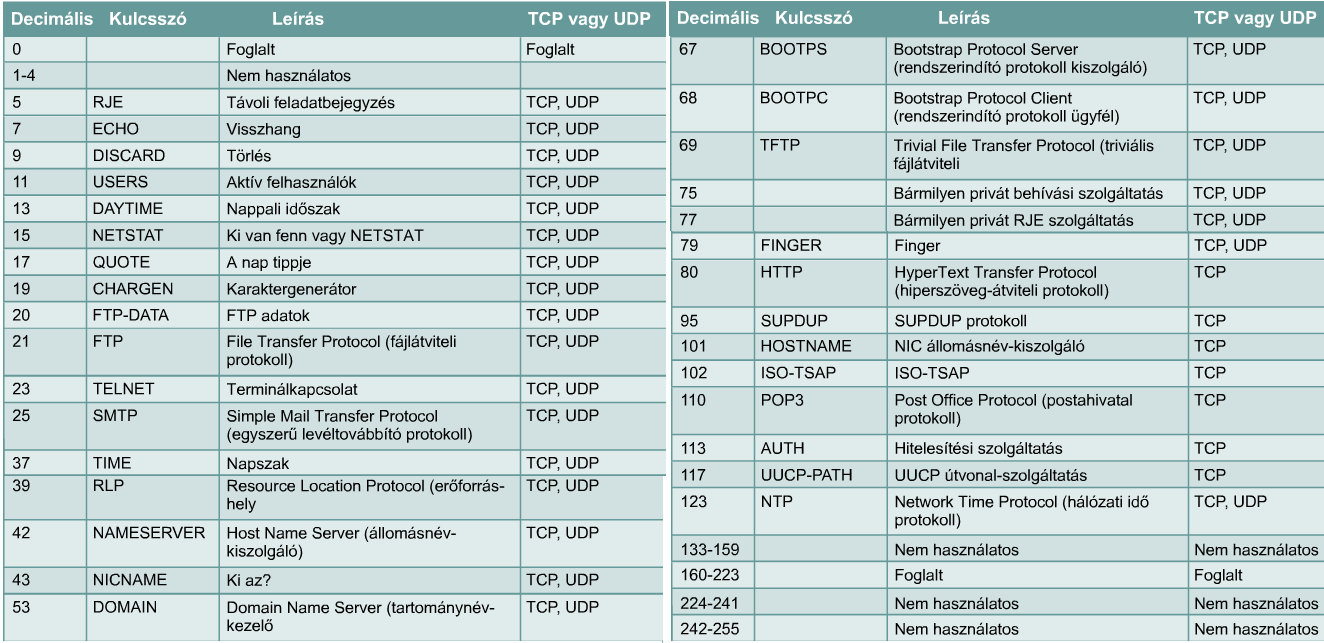
\includegraphics[width=\linewidth]{fig/16-extACL-TCPIP_protocolls}}

A kiterjesztett ACL-ek logikai műveleteket – egyenlő (equal, eq), nem egyenlő (not equal,
neq), nagyobb mint (greater than, gt), kisebb mint (less than, lt) – is képesek végezni a
megadott protokollokon. A kiterjesztett ACL-ek hozzáférési lista száma 100 és 199 között
lehet. (Az újabb IOS-változatoknál a sorszám a 2000–2699 tartományba is tartozhat.)

Az \verb|ip access-group| paranccsal egy meglévő kiterjesztett ACL köthető hozzá egy interfészhez.
Ne feledjük, hogy interfészenként, irányonként és protokollonként csak egy ACL adható meg!
A parancs formátuma: \verb+Router(config-if)#ip access-group hozzáférési-lista-száma {in | out}+
